
The software has three main functionalities, namely, reviewing the GWAS literature, designing prospective association studies, and converting between disease models and canonical parametrizations.
We detail each of the three functionalities of the application, and illustrate with examples.

\subsection{Reviewing reported findings in the GWAS catalog}
\label{sec:review-GWAS-studies}

The ``OR-RAF power diagram'' tab of the application provides a tool for reviewing reported associations from existing studies.
The application calculates statistical power based the core parameters common to models of qualitative traits:

\begin{itemize}
    \item Sample sizes, i.e., the number of cases and controls i.e., $(n_1, n_2)$ or $(\phi, n)$.
    \item The canonical parameters $(f, R)$.
\end{itemize}

Users need only prescribe the sample sizes, by one of two ways provided in the first box, i.e., total sample size + fraction of cases, or number of cases + number of controls.

Statistical power of common association tests, including the likelihood ratio test, chi-square test, Welch's t-test, and the LR test, have the same asymptotic power curves.
This shared power limit is calculated as a function of $f$ and $R$, and visualized as a heatmap referred to as the OR-RAF diagram. 


\bigskip

We provide users the options to load and overlay findings reported in the NHGRI-EBI GWAS Catalog \citep{macarthur2016new}, or upload data from other sources compliant with the Catalog's data format.

The visualization is adaptive and fully interactive.
The initial sample sizes are dynamically adjusted, and automatically determined from texts of the article reporting the user selected loci.
Since the sampling structures are many and varied across different studies, and no uniform reporting format is enforced in the catalog, the initial sample sizes are best estimates from the extracted texts.
Information of the selected loci and the study is also dynamically displayed below the diagram.


\bigskip


The unified power analysis allows us to examine results from different studies employing different models and applicable tests, in the same diagram, with the same power limits.
This allows for a systematic review of reported findings for their statistical validity.
In particular, a reported association predicted to have low power given the study's sample size -- lying in the dark regions of the OR-RAF diagram -- while not impossible, invites further scrutiny.
%\footnote{It should be noted that a reported association predicted to have high power is not automatically accurate, as survival bias induced by multiple testing may inflate the reported $f$ and $R$ estimates.}. 
Studies where reported associations show misalignment with the predicted powered curves should also be further investigated for potential problems in the data curation process.

\begin{figure}
    \centering
    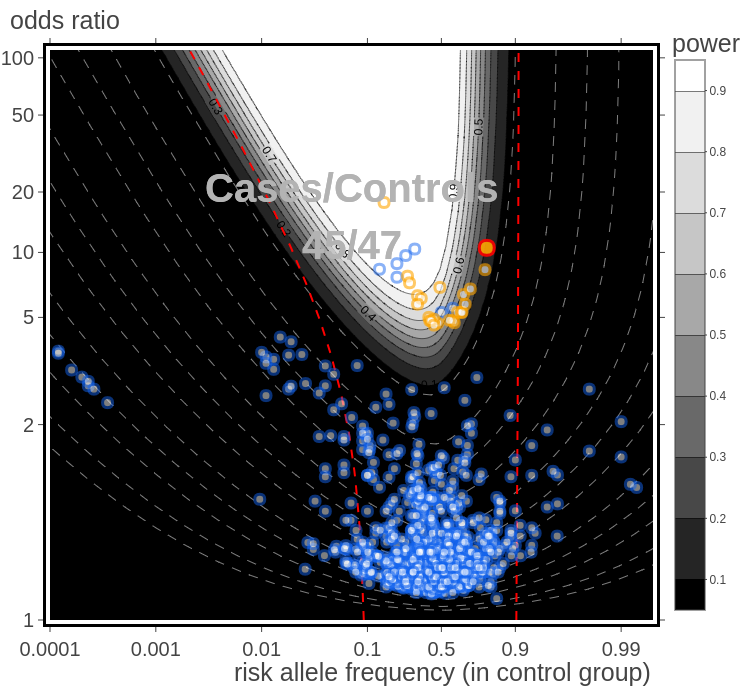
\includegraphics[width=0.49\textwidth]{figures/forensics1.png}
    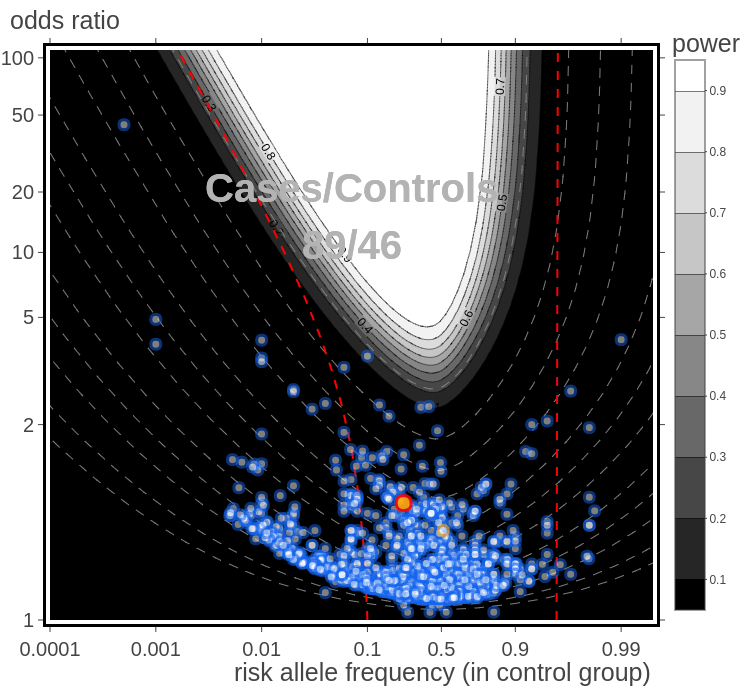
\includegraphics[width=0.49\textwidth]{figures/forensics2.png}
    \caption{The OR-RAF diagram of two studies where gross misalignments were identified. 
    Left: Dominguez-Cruz et al. (2018), right: Haryono et al. (2015). 
    The reported odds ratios and risk allele frequencies of the discovered associations in these two papers are charted with orange (and red) circles. 
    Dark regions represent $f$-$R$ parameter combinations that are predicted to have low power of dicovery under the current sample sizes.
    See text for more comments.}
    \label{fig:forensics}
\end{figure}

We illustrate this forensics feature of the the software with two GWAS studies by \cite{dominguez2018pilot} and \cite{haryono2015pilot}, shown in Figure \ref{fig:forensics}. 
Gross misalignments with our power analysis were identified in both cases.
    Uppon contact, \cite{dominguez2018pilot} confirmed that this misalignment is the result of a problem in the data curation process of the GWAS Catalog (Dominguez-Cruz, personal communication). 
    In particular, the risk allele frequencies reported in the Catalog were based on all subjects in the study, as opposed to only the control group, while the Catalog requires that risk allele frequencies be reported in the control group only. 
    As a consequence, the risk allele frequencies are systematically overestimated, shifting the reported findings to the right in the diagram.
    The study by \cite{haryono2015pilot}, though may very well hold valid results, calls for further scrutiny of its statistical methodologies given the apparent incongruity of its conclusions at the reported the sample sizes.

In general, however, we expect the forensics aspect of our software to be useful for discovering problems with data entry and catalog curation process, as well as for assessing the reproducibility and robustness of reported findings.


\subsection{Designing association studies}
\label{sec:design-my-study}

The ``Design my studies'' tab of the application provides a tool for finding optimal designs of association studies.
The tool requires inputs in a four-step process.
\begin{enumerate}
    \item Model specification.
    \item Sample size constraints specification.
    \item False discovery Criteria specification.
    \item Power specification.
\end{enumerate}
Each of the steps can be specified in a number of alternative ways.

\bigskip
\noindent
{\bf Step 1: Model specification.}
We provide two three ways to describe the model for biological process of the disease or trait of interest.

The distribution of observations can be specified through the canonical parameters, risk allele frequency in the control group ($f$) and odds ratio ($R$).
Estimates for these quantities in previous studies of the same trait can be found in GWAS catalogs such as the NHGRI-EBI Catalog.
See Section \ref{sec:optimal-design} for their definitions.

Alternatively, users may opt to specify through the disease models, of which we implement the four most popular ones: additive, multiplicative, dominant, and recessive.
See Section \ref{sec:power-analysis-overview} below for the definitions of the quantities involved in the disease models.
We remind users the difference between the risk allele frequency in the control group ($f$) versus risk allele frequency in the general population ($p$); only the latter is used in the disease model specifications.

Advanced users may choose to use a more succinct ``signal size per sample'' option, which directly parametrizes the signal sizes ($\lambda/n$).
Definition of signal size $\lambda$ can be found in Section \ref{sec:odds-and-power}.

\bigskip
\noindent
{\bf Step 2: Sample size specifications.}
The second step requires users input the sample size constraints of the study.
The three available options are ``Budget / total number of subjects'', ``Number of cases'', and ``Fraction of cases''.
In the subsequent calculations, the selected and specified quantities are treated as fixed.
With only one unknown parameter left in the flow of power calculations (recall the flowchart in Fig. \ref{fig:flowchart}), we calculate power as a function of the  remaining specified parameter.
In particular,

\begin{itemize}
    \item If the constraint is total budget, power is shown as a function of the fraction of cases.
    \item If the constraint is number of cases, power is shown as a function of the number of controls.
    \item If the constraint is fraction of cases, power is shown as a function of the total number of subjects.
\end{itemize}

\bigskip
\noindent
{\bf Steps 3 and 4: False discovery and power specifications.}
The final two steps require as input the desired level of false discovery and false non-discovery control.
Both specification can be done through the marginal levels, i.e., Type I error and Type II error, or alternatively, through the multiple testing-adjusted levels, i.e., family-wise error rate (FWER) and family-wise non-discovery rate (FWNR).

\begin{figure}
    \centering
    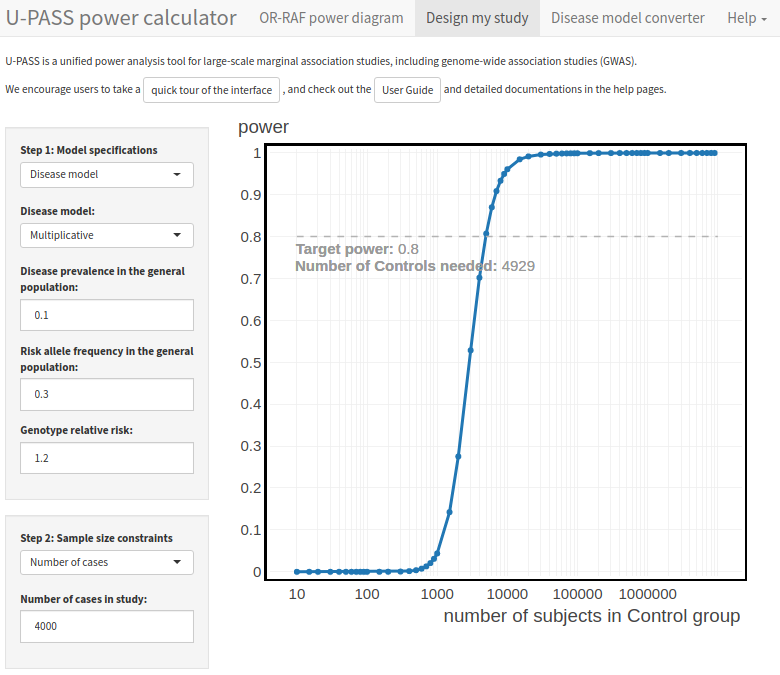
\includegraphics[width=0.8\textwidth]{figures/UPASS_power_analysis.png}
    \caption{A screenshot of the user interface for the ``Design my study'' tab of the software. The inputs are as described in the numerical example in Section \ref{sec:design-my-study}. Results of the power calculation are visualized in an interactive plot in the application.}
    \label{fig:UPASS-power-analysis}
\end{figure}


\bigskip
\noindent
{\bf An example: designing prospective studies.}
A researcher wishes to find out how many controls are needed in order to detect an association between a risk variant described by a multiplicative model with parameters:
$$
\text{GRR} = 1.2, \quad p = 0.3, \quad \text{Prev} = 0.1.
$$
The study has recruited 1000 subjects in the case group, and is aiming for power of 80\% with FWER controlled at 5\% level adjusted for the multiplicity of $10^6$ tests.

In the application, we input the disease model parameters in the first step.
In the second step, we select the sample size constraint as ``number of cases'' and set to 1000.
The third step, we selected FWER as the criteria, and set the appropriate levels and multiplicity; a p-value cut off ($0.05/10^6=5\times10^{-8}$) is automatically calculated and displayed.
The final step, we choose ``Type II error / (1-power)'' as the target and select $1-80\%=20\%$.

The result of the calculation shows that the targeted power cannot be achieved at the current number of cases, no matter how many controls are recruited.
Therefore, the researcher should consider recruiting more subjects in the case group in order to in crease power.
For example, if there are instead 4000 subjects in the case group, then we would need only roughly 4929 controls in order to achieve the desired level of power.


\subsection{Converting disease models into canonical parametrization}

The ``Disease model converter'' tab of the application provides a tool for converting disease models into their implied canonical parameters.
See Figure \ref{fig:UPASS-model-converter} for a screenshot.

\begin{figure}
    \centering
    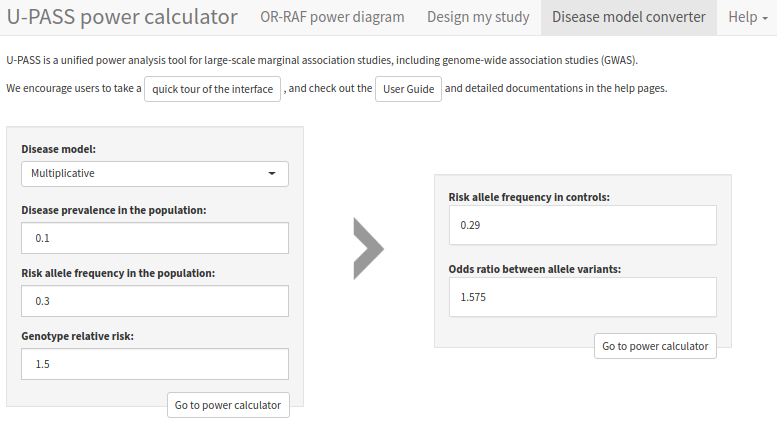
\includegraphics[width=0.8\textwidth]{figures/UPASS_model_converter.png}
    \caption{A screenshot of the user interface for the ``Disease model converter'' tab of the software. See Section \ref{sec:disease-models} for details of the conversion between disease models and canonical parameters in genome-wide association studies.}
    \label{fig:UPASS-model-converter}
\end{figure}

The converter implements the mapping from disease models to the canonical parameters as detailed in Section \ref{sec:disease-models} and  illustrated in Figure \ref{fig:flowchart}.
The tool also allows users to copy the model parameters into the ``Design my study'' tab for power calculations.
Several numerical examples, discussed in Section  \ref{sec:disease-models}, are provided in the tool. 

